\documentclass[10pt]{article}

\usepackage{amsfonts,amssymb}
\usepackage[utf8]{inputenc}
\usepackage[english,russian]{babel}
\usepackage{graphicx}
\usepackage{mathtools}
\usepackage{multicol}
\usepackage{ textcomp }
\usepackage[colorlinks,urlcolor=blue]{hyperref}

\newcommand{\argmin}{\mathop{\rm arg\,min}\limits}
\newcommand{\argmax}{\mathop{\rm arg\,max}\limits}
\newcommand{\sign}{\mathop{\rm sign}\limits}
\newcommand{\cond}{\mspace{3mu}{|}\mspace{3mu}}
\def\RR{\mathbb{R}}
\def\XX{\mathbb{X}}
\def\EE{\mathbb{E}}
\def\NN{\mathcal{N}}
\def\LL{\mathcal{L}}
\def\YY{\mathbb{Y}}

\textheight=220mm
\textwidth=160mm

\title{Школа анализа данных\\ Восстановление зависимостей \\Домашнее задание №1}
\author{Кошман Дмитрий}
\date{}

\begin{document}
	
	
	\voffset=-20mm
	\hoffset=-17mm
	\font\Got=eufm10 scaled\magstep2 \font\Got=eufm10
	
	
	\maketitle
	
	\bigskip
	
	\textbf{Задача 1}
	\medskip
	
	Пусть $C = A^TA + \alpha B^T B$
	
	Поскольку $B$ имеет полный ранг по столбцам, то $Bx \neq 0 \medspace \forall x \Rightarrow ||Bx||  > 0$.
	
	Тогда $x^TCx = x^TA^TAx + \alpha x^tB^T Bx = || Ax || + \alpha || Bx ||  > 0 \forall x$
	
	Значит, $Cx \neq 0 \medspace \forall x$ и $C$ не вырождена.
	
	\bigskip
	
		\textbf{Задача 2}
		
	\medskip
	
	Интегральное уравнение:
	
	$$ \int_{0}^{x}f(t)dt = u(x) ; \medspace u(0) = 0$$
	
	Его решение с точностью до константы:
	
	$$f(x) = u'(x)$$
	
	Рассмотрим случай наблюдаемой функции $u(x)=\sin(2\pi x)$ и ее возмущение функциями
	
	$$\delta_n (x) = \frac {\sin(n^2(x))}{n}; \medspace ||\delta_n(x)|| \rightarrow 0 \text{ при } n \rightarrow \infty :$$
	
	$$ \int_{0}^{x}f_n(t)dt = u(x) + \delta_n(x) \Rightarrow f_n(x) = u'(x)  + \delta_n'(x) = 2\pi \cos(2\pi x) + 2n\cos(n^2 x)$$
	
	Рассмотрим для разных $n$ возмущенную наблюдаемую функцию и ее решение:

	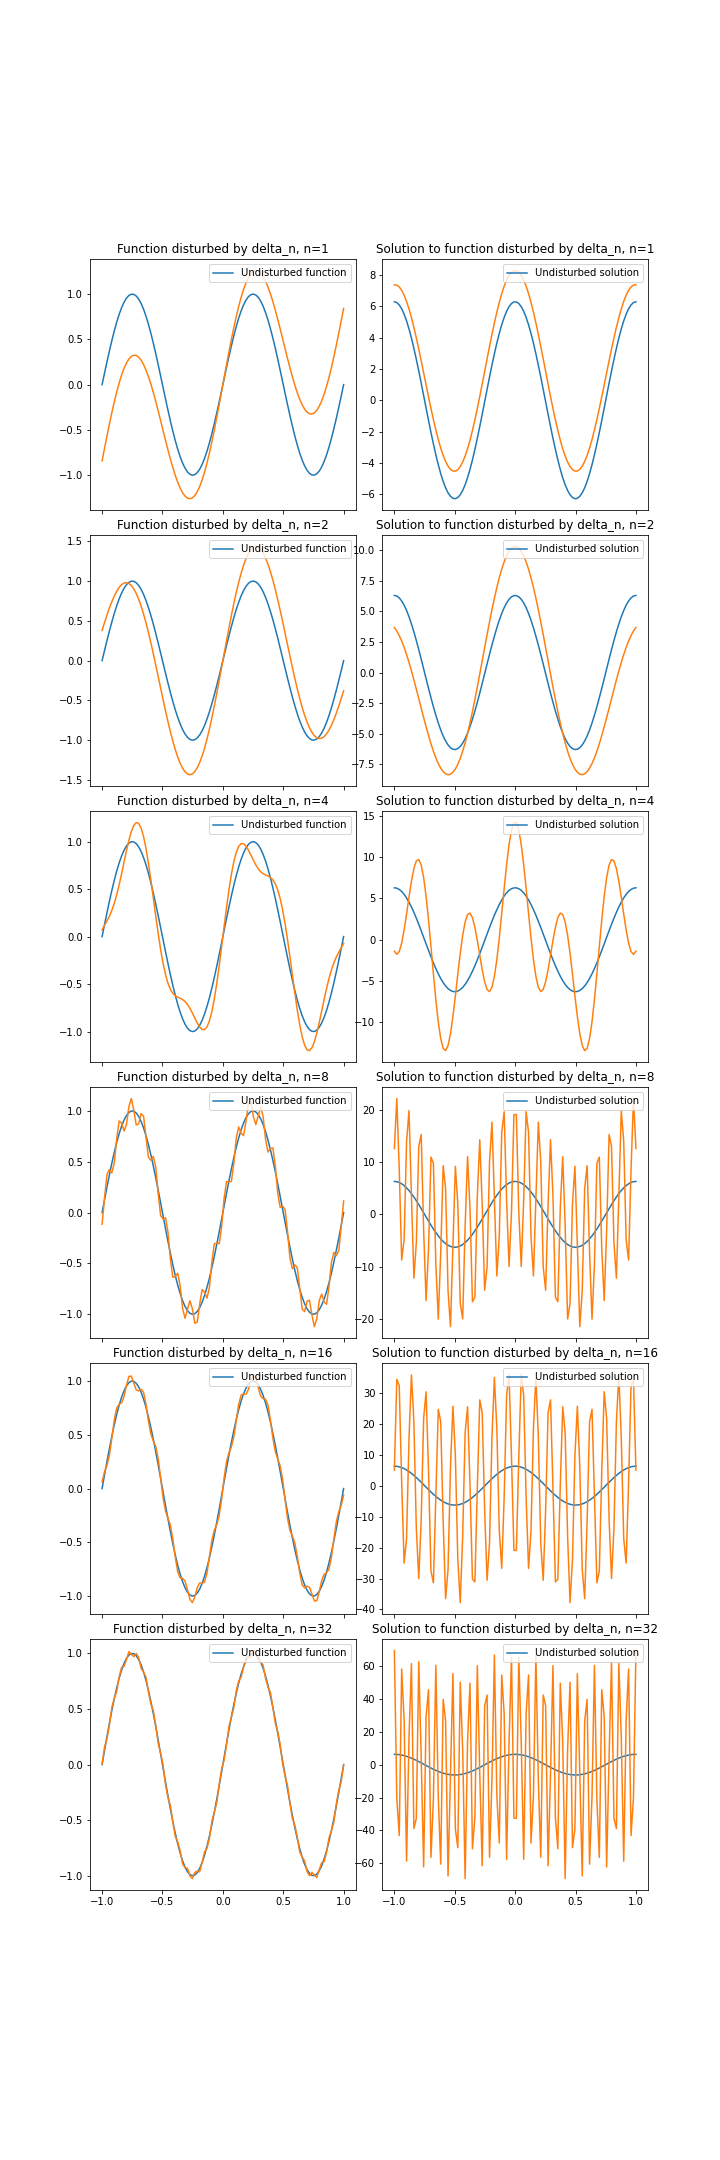
\includegraphics[width=.6\textwidth]{Disturbed solution.png}

	
	\bigskip
	
		\textbf{Задача 3}
		
	\medskip
	
	Будем численно вычислять производную как $u'(x) \approx \hat{u}(x) = \frac{u(x+h) - u(x-h) }{2h} $, причем выбирать шаг дискретизации как $h  = \sqrt{\delta}$, где $\delta$ - величина возмущения.
	
	Покажем, что численная аппроксимация сходится к истинной производной:
	
	$$||\hat{u} - u|| = \max_x |  \frac{u(x+h) - u(x-h) }{2h} - u'(x)| = \max_x |\frac{u'(t) \cdot 2h}{2h} - u'(x)|=\max_x | u'(t) - u'(x) |, $$
	
	Где $t \in  (x-h, x+h) $. Значит, если производная равномерно непрерывна, то $u'(t) \rightarrow u'(x)$ при $h\rightarrow 0$ и $\hat{u} \rightarrow u$.
	
	Также можно оценить погрешность, если вторая производная существует и ограничена: если $|u''(x)| < c$, то 
	
	$$ ||\hat{u} - u|| = \max_x | u'(t) - u'(x) | \leq 2ch$$
	
	Покажем, что $\hat{u}$ устойчива к возмущениям известной величины $\delta$:
	
	$$ ||\hat{ \tilde{u}} -u'|| = ||\frac{\tilde{u}(x+h) - \tilde{u}(x-h) }{2h} -u'(x)|| \leq ||\frac{u(x+h) - u(x-h) }{2h} -u'(x)|| + |\frac{2\delta}{2h}|=$$ 
	
	$$ \max_x | u'(t) - u'(x) | + \sqrt{\delta}$$
	
	Где $t \in  (x-\delta, x+\delta) $. Значит, если $\delta \rightarrow 0$, то $ ||\hat{ \tilde{u}} -u'|| \rightarrow 0$, и решение устойчиво. Проиллюстрируем это графически, выбирая $h = \min\{0.1, \sqrt{\delta}\}$:
	
	\begin{figure}[h]
	 	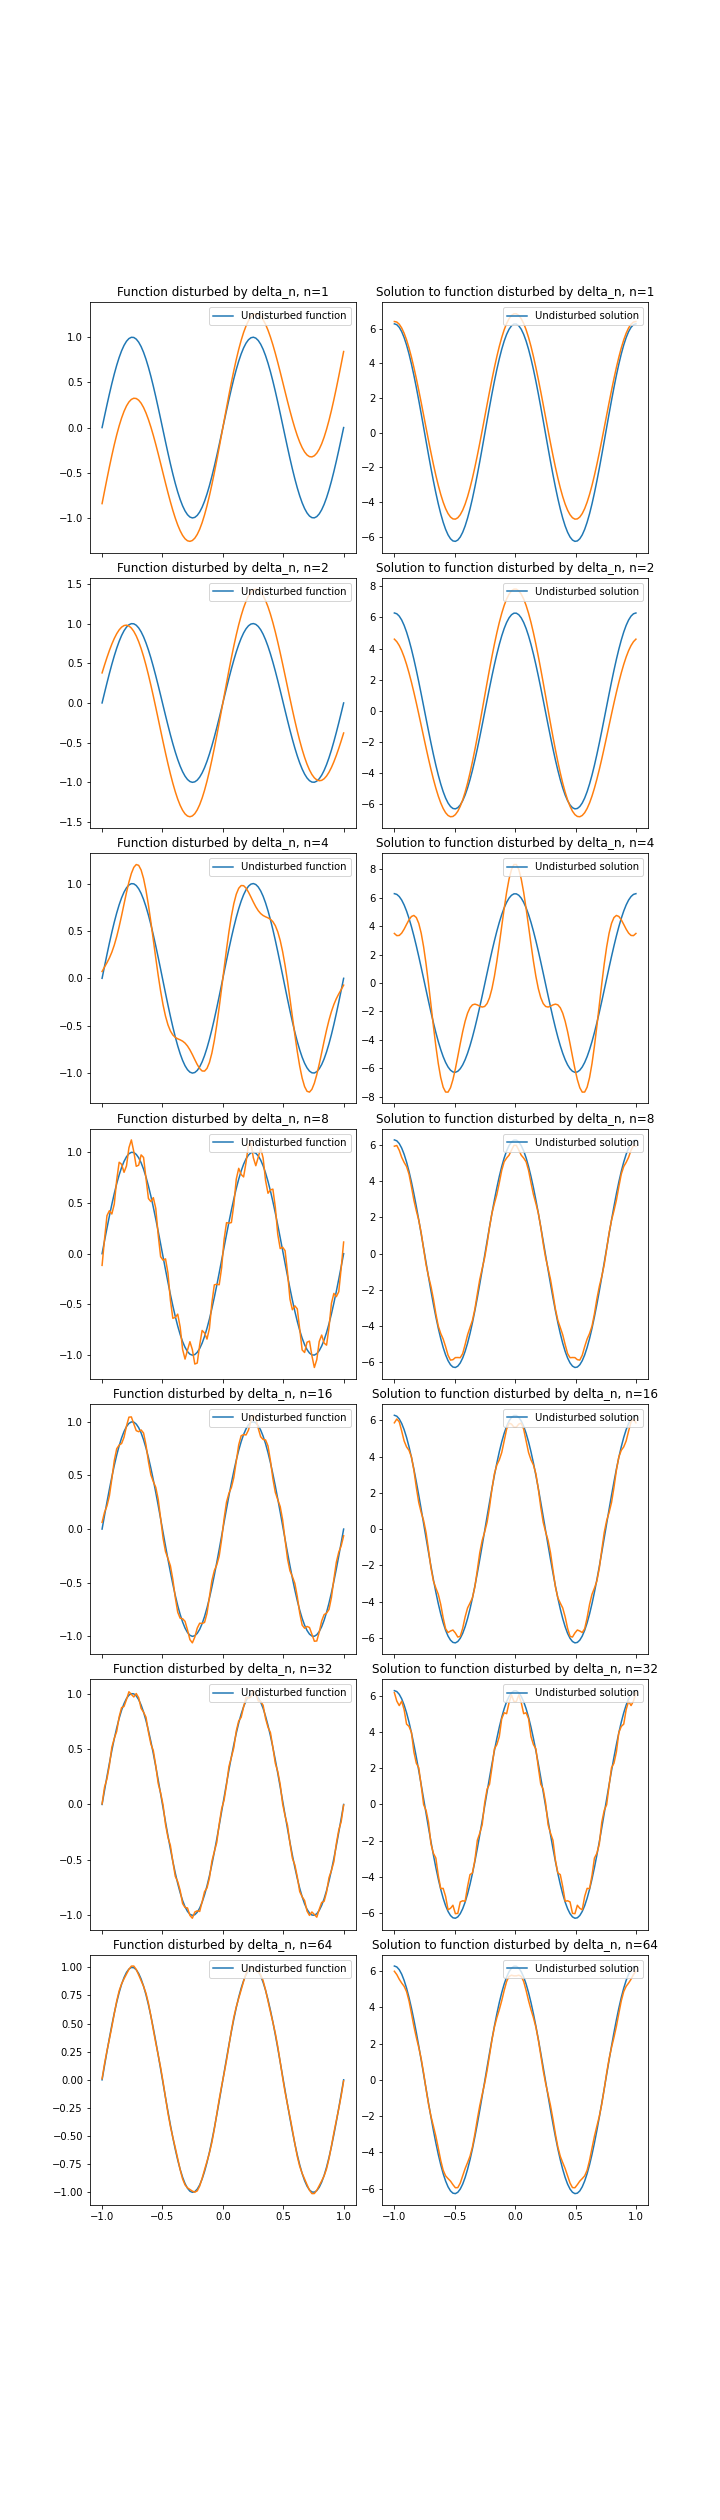
\includegraphics[width=.5\textwidth]{Disturbed solution 2.png}
	\end{figure}	
	
	
	

	
	\bigskip
	
	
	
	
\end{document}

